\documentclass{article}
\usepackage{geometry}
\usepackage{float}
\usepackage[T1]{fontenc}
\usepackage[polish]{babel}
\usepackage[utf8]{inputenc}
\usepackage{graphicx}
\graphicspath{ {./images/} }

\geometry{
 a4paper,
 total={170mm,257mm},
 left=20mm,
 top=20mm,
}

\title{Analiza i przetwarzanie dźwięku - Projekt 2}
\date{04/05/2020}
\author{Mateusz Śliwakowski}

\begin{document}
  \pagenumbering{gobble}
  \maketitle
  \pagenumbering{arabic}
  
\section{Treść zadania}
Celem zadania było zaimplementowanie programu, który wczytuje plik audio a następnie przeprowadza jego analizę widmową. Należało umożliwić użytkownikowi wykonanie transformaty Fouriera całego sygnału oraz ramek o długości $2^N$ zaczynających się w dowolnym miejscu w sygnale. Dla ramek należało umożliwić zastosowanie funkcji okienkowych:
\begin{itemize}
\item okna prostokątnego,
\item okna Hamminga,
\item okna van Hanna.
\end{itemize}
Kolejną funkcjonalnością, którą była wymagana było rysowanie spektogramu dla sygnału. Należało pozwolić na zmianę długości ramek, wybór okna oraz zmianę procentu nakładania się ramek. Ostatnim wymaganiem było zaimplementowanie wykresu częstotliwości krtaniowej za pomocą cepstrum.

\section{Opis aplikacji}

Aplikację zdecydowałem się wykonać w języku \textit{C\#} w środowisku \textit{WinForms}. Całość zacząłem od zaprojektowania wyglądu interfejsu użytkownika.

\begin{figure}[h]
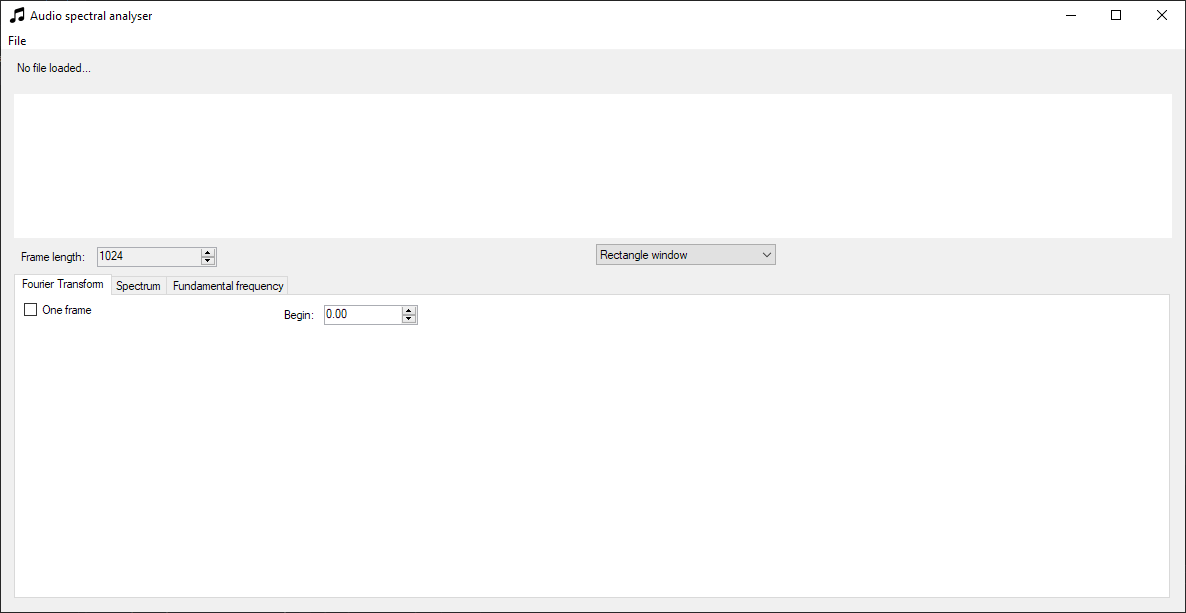
\includegraphics[width=\textwidth]{scr1.png}
\caption{Interfejs użytkownika}
\label{fig:interface}
\end{figure}

Do wczytywania plików audio użyłem biblioteki \textit{NAudio}. Bez problemu umożliwia ona ładowanie przebiegu audio oraz informacji o ścieżce takich jak długość, czy sample rate. Do rysowania wykresów użyłem, w przeciwieństwie do poprzedniego projektu, biblioteki \textit{OxyPlot}, która okazała się dużo bardziej komfortowa w użyciu oraz małym nakładem pracy zapełniła podstawowe funkcjonalnosci takie jak przybliżanie i oddalanie wykresu, przesuwanie, dodawanie etykiet osi. Na początku do obliczania FFT używałem funkcji zaimplementowanych w bibliotece \textit{NUnit}, jednak ze względu na niezadowalające rezultaty zmieniłem ją na \textit{MathNet.Numerics}. Dostarczyła mi ona funkcjonalności wystarczające do obliczania FFT, odwrotnej FFT oraz stosowania okien.

\section{Implementacja}
\subsection{Fourier transform}

\section{Wyniki działania programu}

\section{Wnioski}

\begin{figure}[b]
\centering
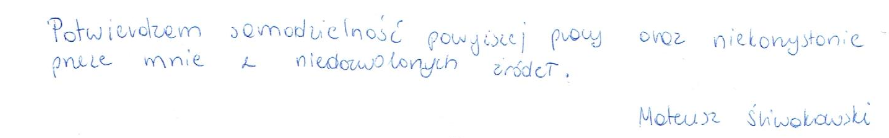
\includegraphics[width=5in]{bottom.png}
\end{figure}

\end{document}

